\section{Wheel Brake System}
\ref{wbs}
To demonstrate the fault modeling capabilities of the Safety Annex we will use the Wheel Brake System (WBS) described in AIR6110~\cite{AIR6110}.  This system is a well-known example that has been used as a case study for safety analysis, formal verification, and contract based design~\cite{DBLP:conf/cav/BozzanoCPJKPRT15, 10.1007/978-3-319-11936-6-7, CAV2015:BoCiGrMa, Joshi05:SafeComp}. The preliminary work for the safety annex was based on a simple model of the WBS~\cite{Stewart17:IMBSA}. To demonstrate a more complex fault modeling process, we constructed a functionally and structurally equivalent AADL version of the more complex WBS NuSMV/xSAP models~\cite{DBLP:conf/cav/BozzanoCPJKPRT15}.    

\begin{figure}[h!]
	\centering
	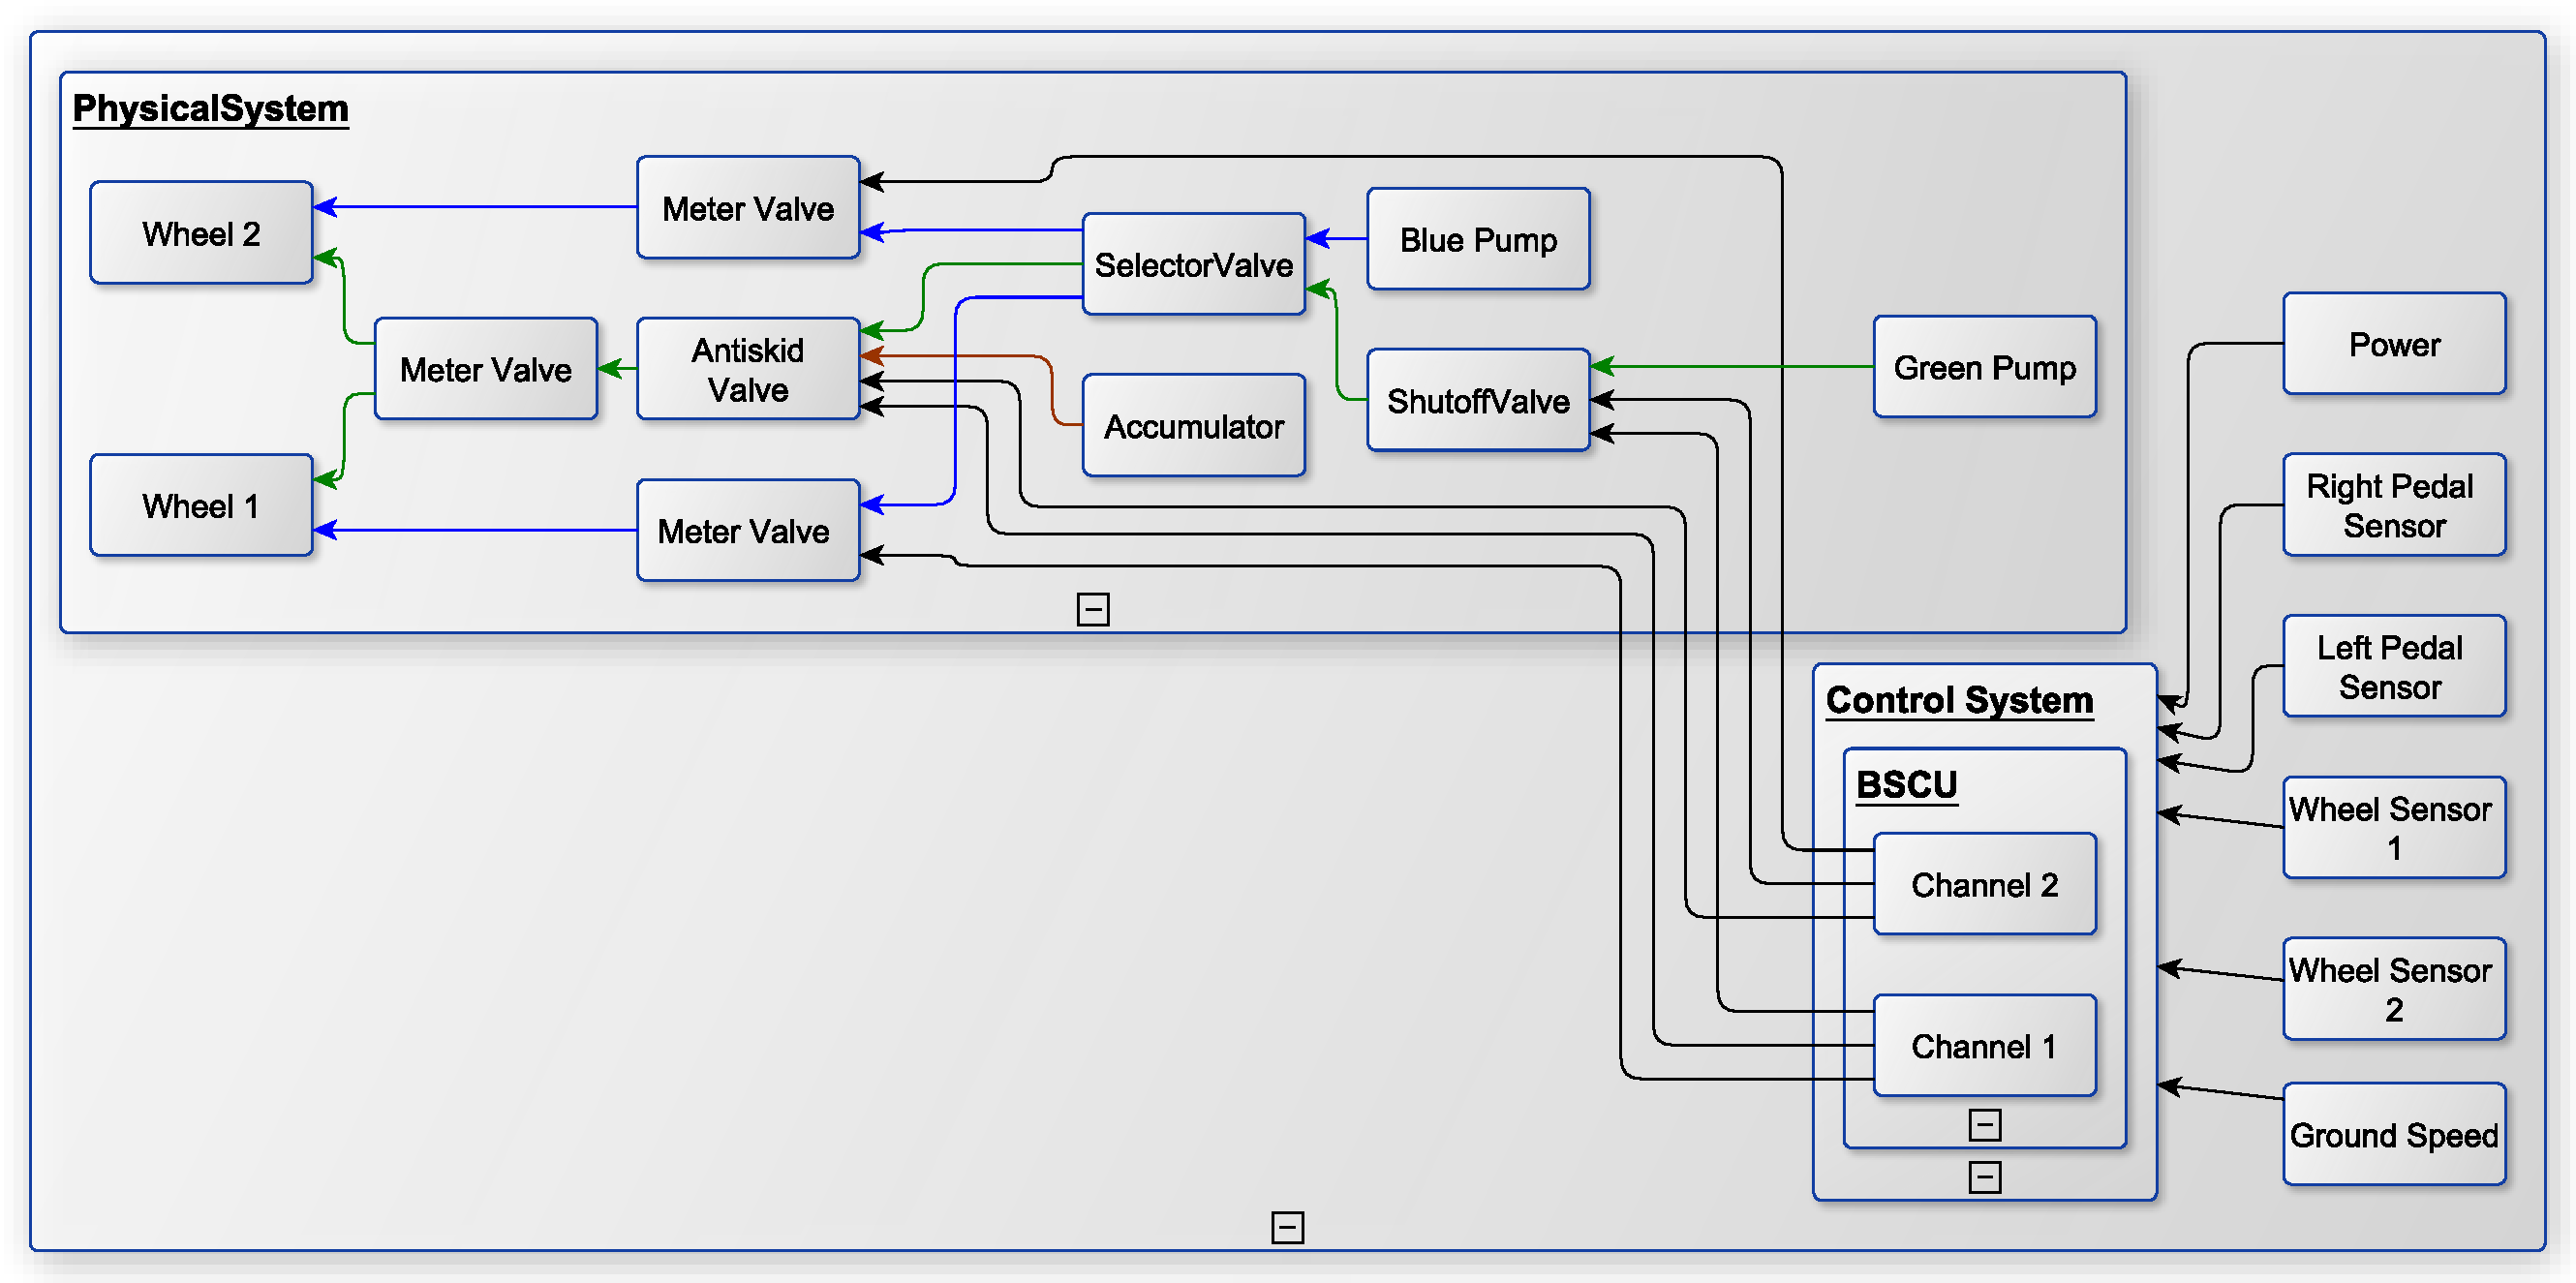
\includegraphics[trim=0 9 0 5,clip,width=\textwidth]{images/wbs_arch4_diagram.pdf}
	\caption{Wheel Brake System}
	\label{fig:wbs}
\end{figure} 

The WBS is composed of two main parts: the Line Replaceable Unit control system and the electro-mechanical physical system.
The control system electronically controls the physical system and contains a redundant
channel of the Braking System Control Unit (BSCU) in case a detectable fault occurs in the active channel.
 It also commands antiskid braking. % in case of skidding on the ground. 
 The physical system consists of the hydraulic circuits running from hydraulic pumps to wheel brakes as well as valves that control the hydraulic fluid flow. This system provides braking force to each of the eight wheels of the aircraft. The wheels are all mechanically braked in pairs (one pair per landing gear). For simplicity, Figure~\ref{fig:wbs} displays only two of the eight wheels. 

There are three operating modes in the WBS model:

\begin{itemize}
	\renewcommand{\labelitemi}{\textbullet}
	\item In \textit{normal} mode, the system is composed of a \textit{green} hydraulic pump and one meter valve per each of the eight wheels. Each of the meter valves are controlled through electronic commands coming from the active channel of the BSCU. These signals provide braking and antiskid commands for each wheel. The braking command is determined through a sensor on the pedal and the antiskid command is determined by the \textit{Wheel Sensors}. 
	\item In \textit{alternate} mode, the system is composed of a \textit{blue} hydraulic pump, four meter valves, and four antiskid shutoff valves, one for each landing gear. The meter valves are mechanically commanded through the pilot pedal corresponding to each landing gear. If the selector detects lack of pressure in the green circuit, it switches to the blue circuit. 
	\item In \textit{emergency} mode, the system mode is entered if the \textit{blue} hydraulic pump fails. The accumulator pump has a reserve of pressurized hydraulic fluid and will supply this to the blue circuit in emergency mode. 
\end{itemize}

The WBS architecture model in AADL contains 30 different kinds of components, 169 component instances, and a model depth of 5 hierarchical levels. 


%If the BSCU channel becomes invalid, the shutoff valve closes and we move into alternate mode. Once this system switches into alternate mode, it does not return to normal operation mode.

%There are three operating modes in the WBS model. In \textit{normal} mode, the system uses the \textit{green} hydraulic circuit. The normal system is composed of the green hydraulic pump and one meter valve per each of the eight wheels. Each of the meter valves are controlled through electronic commands coming from the active channel of the BSCU. These signals provide braking and antiskid commands for each wheel. The braking command is determined through a sensor on the pilot pedal position and is labeled as \textit{Left/Right Pedal Sensor} in Figure~\ref{fig:wbs} and the antiskid command is determined by the \textit{Wheel Sensors}. 

%In \textit{alternate} mode, the system uses the \textit{blue} hydraulic circuit. The alternate system is composed of the blue hydraulic pump, four meter valves, and four antiskid shutoff valves: one for each landing gear. The meter valves are mechanically commanded through the pilot pedal corresponding to each landing gear. If the system detects lack of pressure in the green circuit, the BSCU channel commands the selector valve to switch to the blue circuit. 
%If the BSCU channel becomes invalid, the shutoff valve closes and we move into alternate mode. Once this system switches into alternate mode, it does not return to normal operation mode.

%The last mode of operation of the WBS is the \textit{emergency} mode. This mode is entered if the blue hydraulic pump fails. The accumulator pump has a reserve of pressurized hydraulic fluid and will supply this to the blue circuit in emergency mode.

%The model contains 30 different kinds of components, 169 component instances, a model depth of 5 hierarchical levels.  The model includes one top-level assumption and  11 top-level system properties, with 113 guarantees allocated to subsystems.  There are a total of 33 different fault types and 141 fault instances within the model.  The large number of fault instances is due to the redundancy in the system design and its replication to control 8 wheels.

The behavioral model is encoded using the AGREE annex and the behavior is based on descriptions found in AIR6110. The top level system properties are given by the requirements and safety objectives in AIR6110. All of the subcomponent contracts support these system safety objectives through the use of assumptions on component input and guarantees on the output. The WBS behavioral model in AGREE annex includes one top-level assumption and  11 top-level system properties, with 113 guarantees allocated to subsystems.  

An example system safety property is to ensure that there is no inadvertent braking of any of the wheels. This is based on a failure condition described in AIR6110 is \textit{Inadvertent wheel braking on one wheel during takeoff shall be less than 1E-9 per takeoff}. 
Inadvertent braking means that braking force is applied at the wheel but the pilot has not pressed the brake pedal.  In addition, the inadvertent braking requires that power and hydraulic pressure are both present, the plane is not stopped, and the wheel is rolling (not skidding). The property is stated in AGREE such that inadvertent braking does \textit{not} occur, as shown in Figure \ref{fig:inadvertent_braking}. 

\begin{figure}[h!]
	%\vspace{-0.2in}
	\begin{center}
		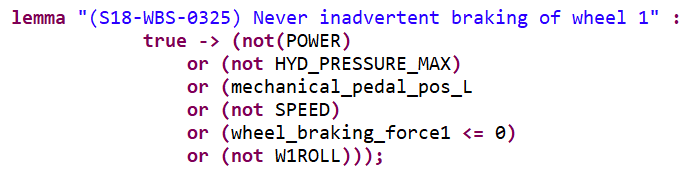
\includegraphics[width=.7\textwidth]{images/inadvertent_braking.png}
	\end{center}
	\vspace{-0.3in}
	\caption{AGREE Contract for Top Level Property: Inadvertent Braking}
	\label{fig:inadvertent_braking}
	%\vspace{-0.2in}
\end{figure}